
%(BEGIN_QUESTION)
% Copyright 2007, Tony R. Kuphaldt, released under the Creative Commons Attribution License (v 1.0)
% This means you may do almost anything with this work of mine, so long as you give me proper credit

From Bernoulli's equation, develop a formula for calculating volumetric flow rate ($Q$) given differential pressure drop $\Delta P$ between two flow streams with differing cross-sectional areas ($A_1$ and $A_2$).  Assume an incompressible fluid ($\rho$ = constant) flowing along a level path ($z_1 = z_2$), and recall that volumetric flow rate is equal to the product of cross-sectional area and fluid velocity ($Q = Av$).

$$\includegraphics[width=15.5cm]{i02983x01.eps}$$

\vskip 10pt

\noindent
{\bf Bernoulli's equation:}

$$z_1 \rho g + {v_1^2 \rho \over 2} + P_1 = z_2 \rho g + {v_2^2 \rho \over 2} + P_2$$


\underbar{file i02983}
%(END_QUESTION)





%(BEGIN_ANSWER)

Assuming no difference in height ($z$):

$${v_1^2 \rho \over 2} + P_1 = {v_2^2 \rho \over 2} + P_2$$

$$P_1 - P_2 = {v_2^2 \rho \over 2} - {v_1^2 \rho \over 2}$$

$$\Delta P = {\rho \over 2} \left( v_2^2 - v_1^2 \right)$$

$${2 \Delta P \over \rho}= v_2^2 - v_1^2$$

$$\hbox{If } Q = Av \hbox{ then } v = {Q \over A}$$

$${2 \Delta P \over \rho} = \left({Q \over A_2}\right)^2 - \left({Q \over A_1}\right)^2$$

$${2 \Delta P \over \rho} = {Q^2 \over A_2^2} - {Q^2 \over A_1^2}$$

$${2 \Delta P \over \rho} = {Q^2 A_1^2 \over A_1^2 A_2^2} - {Q^2 A_2^2 \over A_1^2 A_2^2}$$

$${2 \Delta P \over \rho} = Q^2 {A_1^2 - A_2^2 \over A_1^2 A_2^2}$$

$$Q^2 = \left({A_1^2 A_2^2 \over A_1^2 - A_2^2}\right) \left({2 \Delta P \over \rho}\right)$$

$$Q = \sqrt{A_1^2 A_2^2 \over A_1^2 - A_2^2} \> \sqrt{2 \Delta P \over \rho}$$

$$Q = {A_1 A_2 \over \sqrt{A_1^2 - A_2^2}} \> \sqrt{2 \Delta P \over \rho}$$


\noindent
Where,

$Q$ = Volumetric flow rate (ft$^{3}$/s)

$A_1$ = Large flow area (ft$^{2}$)

$A_2$ = Small (throat) flow area (ft$^{2}$)

$\Delta P$ = Differential pressure drop (lb/ft$^{2}$)

$\rho$ = Mass density of fluid (slugs/ft$^{3}$)

\vskip 10pt

%(END_ANSWER)





%(BEGIN_NOTES)

%INDEX% Physics, dynamic fluids: Bernoulli's equation

%(END_NOTES)


